\documentclass{jsarticle}
\usepackage[dvipdfmx]{graphicx}
\usepackage{amsmath,amssymb}
\usepackage{mathtools}
\mathtoolsset{showonlyrefs=true}

\title{やさしく学ぶ機械学習を理解するための数学のきほん}

\begin{document}

\maketitle
\section{イントロダクション}

\subsection{機械学習が得意とすること}

\begin{itemize}
	\item{回帰(Regression)}
    \item{分類(Classification)}
    \item{クラスタリング(Clustering)}
\end{itemize}

\subsubsection{回帰}
連続するデータ(例えば時系列データなど)を扱うときに使われる

株価のような過去のデータが入手できるもので、「明日の株価はどうなりそうか」などを予測するのに回帰を使うことがある。

\subsubsection{分類}
例えばスパムメールの判定などに使われる。

スパムかどうかなどの分類先が二つしかないものは二値分類と呼ばれ、3つ以上の場合は多値分類と呼ばれる。数字の識別は多値分類に相当する。

\subsubsection{クラスタリング}
例えば生徒が100人いる学校の学力テストがあったとする。そのテストの点数によって生徒100人を幾つかのグループに分けるような問題のこと。

分類に似ているが、違うのはデータにラベルが付いていないということ。スパムメール判定で、メールの内容と一緒に、そのメールがスパムかどうかというラベルが付与されていた。でもテストの点数のデータに分類に関するラベルは付いていない。

ラベルが付いているデータを学習することを教師あり学習、ラベルが付いていないデータを使って学習することを教師なし学習という。回帰と分類は教師あり学習、クラスタリングは教師なし学習と言える。

\section{回帰}
以下の図のように年齢と年収のデータがあったとする(ドット)。このデータに近似するように一次関数の線を引くことができる(赤線)。

\begin{center}
  \includegraphics[width=15cm]{figures/kaiki.png}
\end{center}

ここで赤線の関数を以下の式と定義する。

\[
	f(\theta) =  \theta_0  + \theta_1 x
\]

$\theta$は未知数(パラメータ)の事。統計学の世界では未知数や推定値を$\theta$で表すことが多い。

\subsection{最小二乗法}
$\theta$の値を実データとの誤差が採用になるように求める必要がある。誤差が0になるのが理想だが、すべてのデータに対して誤差を0にするのは不可能なので、すべてのデータの誤差の合計がなるべく小さくなるようにする。

実データがn個あるとして、実データごとの誤差の総和は以下のように表すことができる。

\[
	E(\theta) = \frac{1}{2} \sum_{i=1}^n(y^{(i)}-f_{\theta}(x^{(i)}))^{2}
\]

$y^{(i)}$などはi乗という意味ではなく、i番目の実データという意味。

各データごとの誤差を2乗してそれを全部足し、$ \frac{1}{2}$ してあげることで、E($\theta$)の値が一番小さくなるような$\theta$を見つけることが目的。こういうものを\bf{最適化問題}という。

絶対値でなく2乗することも、$\frac{1}{2}$をかけるのも、あとあと微分する時に計算を楽にするため。

こういうアプローチのことを\bf{最小二乗法という}

\subsection{最急降下法}
$\theta$の値を適当に変えながらE($\theta$)を計算し行くのは面倒。微分を使って求めていく。

微分について簡単に、$g(x)=(x-1)^{2}$を例に見ていく。

\begin{center}
  \includegraphics[width=15cm]{figures/grah2.png}
\end{center}

展開すると$(x-1)^{2}=x^{2}-2x+1$であり、微分すると$\frac{d}{dx}g(x)=2x-2$。どう関数の値を小さくなるようにxの値を更新する。これを\bf{最急降下法}や\bf{勾配降下法}と呼ぶ。以下を更新式とする。

\[
	x := \eta\frac{d}{dx}g(x)
\]

$A := B$は「AをBによって定義する」という意味。$\eta$は「学習率」と呼ばれる正の定数。学習率の大小によって、最初うちにたどり着くまでの更新回数が変わってくる。収束の速さが変わるともいう。

目的関数E($\theta$)に話を戻すと、E($\theta$)はg(x)と同様に下に凸の形をしているから同じ議論を当てはめることができる。ただ、この目的関数は$\theta_0$と$\theta_1$の二つの変数を含んでいるから、普通の微分ではなくて偏微分になっている。更新式は以下のようになる

\[
	\theta_0 := \theta_0 - \eta \frac{\partial E}{\partial \theta_0} 
    \hspace{15pt}
    \theta_1 := \theta_1 - \eta \frac{\partial E}{\partial \theta_1}
\]

E($\theta$)を偏微分してみる。E($\theta$)の中に$f_{\theta}(x)$が出てきて$f_{\theta}(x)$の中に$\theta_{0}$が出てくるので、それぞれ以下のように考える。

\[
	u = E(\theta)
    \hspace{15pt}
    v = f_{\theta}(x)
\]

すると段階的に微分することができる。

\[
	\frac{\partial u}{\partial \theta_{0}} = \frac{\partial u}{\partial v} \cdot \frac{\partial v}{\partial \theta_{0}}
\]

まずはuをvで微分する。

\begin{align}
	\frac{\partial u}{\partial v} &= \frac{\partial}{\partial v}(\frac{1}{2}\sum_{i=1}^n(y^{(i)}-v)^{2})\\
    &= \frac{1}{2}\sum_{i=1}^{n}(\frac{\partial}{\partial v}(y^{i}-v)^{2})\\
    &= \frac{1}{2} \sum_{i=1}^{n} (y^{(i)^{2}} - 2y^{(i)}v + v^{2}))\\
    &= \frac{1}{2} \sum_{i=1}^{n} (-2y^{(i)} + 2v)\\
    &= \sum_{i=1}^{n} (v-y^{(i)})\\
\end{align}

次にvを$\theta_0$で微分する。

\begin{align}
	\frac{\partial v}{\partial \theta_0} = \frac{\partial}{\partial \theta_0} (\theta_0 + \theta_1 x)
    = 1
\end{align}

以上より、$\frac{\partial u}{\partial \theta_{0}} = \frac{\partial u}{\partial v} \cdot \frac{\partial v}{\partial \theta_{0}}$が求まる。

\begin{align}
	\frac{\partial u}{\partial \theta_{0}} &= \frac{\partial u}{\partial v} \cdot \frac{\partial v}{\partial \theta_{0}}\\
    &= \sum_{i=1}^{n} (v-y^{(i)}) \cdot 1\\
    &= \sum_{i=1}^{n} (f_\theta(x^{(i)}) - y^{(i)})
\end{align}

同様の処理を$\theta_1$にも行うと、それぞれの更新式は以下のようになる。

\begin{align}
	\theta_0 *= \theta_0 - \eta \sum_{i=1}^{n} (f_\theta(x^{(i)}) - y^{(i)})\\
    \theta_1 *= \theta_1 - \eta \sum_{i=1}^{n} (f_\theta(x^{(i)}) - y^{(i)}) x^{(i)}
\end{align}

この式にしたがって$\theta_0$と$\theta_1$を更新していけば正しい形の1次関数$f_{\theta}(x)$が見つかる。


\section{多項式回帰}
上記で挙げた一次関数の形よりも曲線のほうがフィットする場合がある。

\begin{center}
  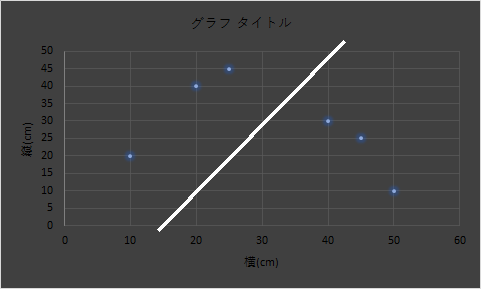
\includegraphics[width=10cm]{figures/graph2.png}
\end{center}

これは関数$f_\theta(x)$を二次関数として定義することで実現できる。

\begin{align}
	f_{\theta}(x) = \theta_0 + \theta_1 x + \theta_2 x^{2}
\end{align}

もしくはもっと大きな字数を持った式にしても適応できる。

\begin{align}
	f_{\theta}(x) = \theta_0 + \theta_1 x + \theta_2 x^{2} + ・・・  + \theta_n x^{n}
\end{align}

次数を増やせば増やすほどフィッットするようにはなるが、「過学習」と呼ばれる避けては通れない別の問題が発生する。

二次関数の場合の更新式は以下のようになる。

\begin{align}
	\theta_0 = \theta_0 - \eta \sum_{i=1}^{n} (f_\theta(x^{(i)}) - y^{(i)})\\
    \theta_1 = \theta_1 - \eta \sum_{i=1}^{n} (f_\theta(x^{(i)}) - y^{(i)}) x^{(i)}\\
    \theta_2 = \theta_1 - \eta \sum_{i=1}^{n} (f_\theta(x^{(i)}) - y^{(i)}) x^{(i)^{2}}
\end{align}

このように、パラメータが$\theta_3,\theta_4$と増えていっても同じことをして更新式を求めることができる。多項式の次数を増やした関数を使うものは、「多項式回帰」と呼ばれる。


\section{重回帰}
解きたい問題の多くは、変数が2つ以上の複雑な問題のことが多い。

例えば、「広告費用の金額によってクリック数が決まる」と設定すると、単純に広告費用に比例したクリック数となるが、現実問題、クリック数は様々な要因で上下する。例えば、広告の位置であったりサイズであったり。複数の要素がクリック数に影響を及ぼす。

具体的に「広告費$=x_1$」「広告の横幅$=x_2$」「広告の縦幅$=x_3$」の3つのパラメータで考えると、以下のように表すことができる。

\begin{align}
	f_\theta(x_1,x_2,x_3) = \theta_0 + \theta_1 x_1 + \theta_2 x_2 + \theta_3 x_3
\end{align}

この時のパラメータ$\theta_0,・・・,\theta_3$は、それぞれ偏微分してパラメータを更新すれば求めることができる。

上記式を一般化して

\begin{align}
	f_\theta(x_1,・・・,x_n) = \theta_0 + \theta_1 x_1 + \theta_2 x_2 + ・・・ + \theta_n x_n
\end{align}

と表すことができる。上記のように毎回n個のxを書いていくのは大変なので、パラメータ$\theta$と変数xをベクトルとみなす。

\begin{align}
  	\bf{\theta} = \begin{pmatrix} 
      \theta_0\\
      \theta_1\\
      \vdots\\
      \theta_n
	\end{pmatrix}
    \hspace{15pt}
    \bf{x} = \begin{pmatrix} 
      1\\
      x_1\\
      \vdots\\
      x_n
	\end{pmatrix}
\end{align}

ベクトルxに1を追加しているのは、この方が自然だから。$\theta$の添字が0から始まっているので、それと合わせるために$x_0=1$として、\bf{x}の最初の要素に$x_0$をおく方が綺麗。

\begin{align}
  	\bf{\theta} = \begin{pmatrix} 
      \theta_0\\
      \theta_1\\
      \vdots\\
      \theta_n
	\end{pmatrix}
    \hspace{15pt}
    \bf{x} = \begin{pmatrix} 
      x_0\\
      x_1\\
      \vdots\\
      x_n
	\end{pmatrix}
    (x_0 = 1)
\end{align}	

$\theta$を転置したものと\bf{x}をかけたものを見てみると

\begin{align}
	\bf{\theta^{T}}\bf{x} = \theta_0 x_0 + \theta_1 x_1 + \theta_2 x_2 + \cdots + \theta_n x_n 
\end{align}

と、ベクトル表記する前の式となる。ベクトル式だと、

\begin{align}
	f_{\theta}(\bf{x}) = \bf{\theta^{T}}\bf{x}
\end{align}

次に、この$f_{\theta}(\bf{x})$を使ってパラメータの更新式を求める。$u = E(\theta), v = f_{\theta}(x)$とおくのは同じ。一般化して考えるためにj番目の要素の$\theta_j$で偏微分すると、

\begin{align}
	\frac{\partial u}{\partial \theta_j} = \frac{\partial u}{\partial v} \cdot \frac{\partial v}{\partial \theta_j}
\end{align}

vを$\theta_j$で微分すると、

\begin{align}
	\frac{\partial v}{\partial \theta_j} &= \frac{\partial}{\partial \theta_j}(\bf{\theta}^{T}\bf{x})\\
    &= \frac{\partial}{\partial \theta_j} (\theta_0 x_0 + \theta_1 x_1 + \cdots + \theta_n x_n)\\
    &= x_j
\end{align}

最終的に、j番目のパラメータの更新式は以下のようになる。

\begin{align}
	\theta_j := \theta_j - \eta \sum_{i=1}^n (f_{\theta}(\bf{x}^{(i)}) - y^{(i)})x_j^{(i)}
\end{align}

このように複数の変数を使ったものを「重回帰」という。

\section{確率的勾配降下法}
最急降下法には、計算に時間がかかる以外にも、局所解に捕まってしまうという欠点がある。

最急降下法で関数の最小値を見つけるにしても、まず最初にどのxからスタートするかを決める必要がある。多くは乱数を使ってスタート位置を決めるが、初期位置が不適当な場合、最小値でない部分に落ち着いてしまうことがある。これを「局所解に捕まる」と表現する。

最急降下法のパラメータ更新式、

\begin{align}
	\theta_j := \theta_j - \eta \sum_{i=1}^{n} (f_{\theta}(\bf{x}^{(i)}) - y^{(i)})x_{j}^{(i)}
\end{align}

は、すべての学習データの誤差を使っているが、確率的勾配降下法ではランダムに学習データを1つ選んで、それをパラメータの更新に使う。この式のkはランダムに選ばれたインデックスのことである。

\begin{align}
	\theta_j := \theta_j - \eta (f_{\theta}(\bf{x}^{(k)}) - y^{(k)})x_{j}^{(k)}
\end{align}

ランダムで選ぶデータの数は1つ以上でも構わない。m個選んだ場合は、インデックスの集合をK遠くと以下のようにパラメータを更新する。

\begin{align}
	\theta_j := \theta_j - \eta \sum_{k \in K}^{n} (f_{\theta}(\bf{x}^{(k)}) - y^{(k)})x_{j}^{(k)}
\end{align}

この方法を「ミニバッチ法」という。


\end{document}